% Copyright 2004 by Till Tantau <tantau@users.sourceforge.net>.
%
% In principle, this file can be redistributed and/or modified under
% the terms of the GNU Public License, version 2.
%
% However, this file is supposed to be a template to be modified
% for your own needs. For this reason, if you use this file as a
% template and not specifically distribute it as part of a another
% package/program, I grant the extra permission to freely copy and
% modify this file as you see fit and even to delete this copyright
% notice. 

\documentclass{beamer}

% There are many different themes available for Beamer. A comprehensive
% list with examples is given here:
% http://deic.uab.es/~iblanes/beamer_gallery/index_by_theme.html
% You can uncomment the themes below if you would like to use a different
% one:
%\usetheme{AnnArbor}
%\usetheme{Antibes}
%\usetheme{Bergen}
%\usetheme{Berkeley}
%\usetheme{Berlin}
%\usetheme{Boadilla}
%\usetheme{boxes}
%\usetheme{CambridgeUS}
%\usetheme{Copenhagen}
%\usetheme{Darmstadt}
%\usetheme{default}
%\usetheme{Frankfurt}
%\usetheme{Goettingen}
%\usetheme{Hannover}
%\usetheme{Ilmenau}
%\usetheme{JuanLesPins}
%\usetheme{Luebeck}
%\usetheme{Madrid}
%\usetheme{Malmoe}
%\usetheme{Marburg}
%\usetheme{Montpellier}
%\usetheme{PaloAlto}
%\usetheme{Pittsburgh}
%\usetheme{Rochester}
%\usetheme{Singapore}
%\usetheme{Szeged}
%\usetheme{Warsaw}


% Customizações de Cores: fg significa cor do texto e bg é cor do fundo
\setbeamercolor{normal text}{fg=black}
\setbeamercolor{alerted text}{fg=red}
\setbeamercolor{author}{fg=black}
\setbeamercolor{institute}{fg=blue}
\setbeamercolor{date}{fg=blue}
\setbeamercolor{frametitle}{fg=white}
\setbeamercolor{framesubtitle}{fg=white}
\setbeamercolor{block title}{bg=red, fg=white}		%Cor do título
\setbeamercolor{block body}{bg=gray, fg=darkgray}	%Cor do texto (bg= fundo; fg=tex
%\usepackage{beamerthemeshadow} %Formatação do plano de fundo
%\setbeamercovered{transparent} %Formatação do plano de fundo

\usetheme[secheader]{Boadilla} 
\usecolortheme{seahorse}


\newcommand{\Real}{\mathbb{R}}
\newcommand{\D}{\mathcal{D}}
\newcommand{\Natural}{\mathbb{N}}
\newcommand{\Integer}{\mathbb{Z}}
\newcommand{\Complex}{\mathbb{C}}
\newcommand{\C}{\mathcal{C}}
\newcommand{\N}{\mathcal{N}}

\newcommand{\T}{^{\scriptscriptstyle\rm T}}
\font\bbfnt=msbm10
\def\bbR{\mbox{\bbfnt R}}
\def\bbN{\mbox{\bbfnt N}}
\def\bbZ{\mbox{\bbfnt Z}}
\renewcommand{\(}{\left(}
\renewcommand{\)}{\right)}
\renewcommand{\[}{\left[}
\renewcommand{\]}{\right]}
\newcommand{\SE}{\mathcal{E}}
\newcommand{\isdef}{~\stackrel{\triangle}{=}~}

\usepackage[brazil]{babel}
\usepackage[utf8]{inputenc}
\usepackage{booktabs}
\usepackage[scale=2]{ccicons}
\usepackage{pgfplots}
\usepackage{xspace}
\usepackage{enumerate}
\usepackage{amsthm}
\usepackage[alf]{abntex2cite}
%\usepackage{subcaption}
%\usepgfplotslibrary{dateplot}
\usepackage{graphicx}
\usepackage{mathtools}
%\DeclarePairedDelimiter\abs{\lvert}{\rvert}%
%\usepackage{latexsym}
%\usepackage{amsmath}
%\usepackage[T1]{fontenc}
%\usepackage{fetamont}
%\usepackage{mathrsfs}
\usepackage{subfigure}
%\usepackage{chngcntr}
%\usepackage{fancyhdr}
%\usepackage{xmpmulti}
%\usepackage{animate}
\usepackage{ragged2e}
\usepackage{pdfpages}
\usepackage{epstopdf}
\usepackage{textpos}

\usepackage{adjustbox}
\usepackage{tikz}
\usetikzlibrary{shapes.geometric, arrows, positioning, calc}

\tikzstyle{startstop} = [rectangle, rounded corners, minimum width=3cm, minimum height=1cm,text centered, draw=black, fill=red!30]
\tikzstyle{io} = [trapezium, trapezium left angle=70, trapezium right angle=110, minimum width=3cm, minimum height=1cm, text centered, draw=black, fill=blue!30]
\tikzstyle{process} = [rectangle, minimum width=3cm, minimum height=1cm, text centered, draw=black, fill=orange!30]
\tikzstyle{decision} = [diamond, minimum width=3cm, minimum height=1cm, text centered, draw=black, fill=green!30]
\tikzstyle{arrow} = [thick,->,>=stealth]

\setbeamertemplate{caption}[numbered]
%\setbeamertemplate{footline}[]{}
\setbeamertemplate{navigation symbols}{}
\setbeamertemplate{caption}{\raggedright\insertcaption\par}

\newtheorem{definicao}{}

\setbeamercolor{title}{fg=red!70!black}
\setbeamercolor{subtitle}{fg=black!100}
\setbeamercolor{author}{fg=blue!50!black}
\setbeamercolor{institute}{fg=blue!70!black}
\setbeamercolor{frametitle}{fg=red!90!black}
\setbeamercolor{framesubtitle}{fg=red!80!green!50}
\titlegraphic{
	\vspace{-0.5cm}
	\includegraphics[width = 1.5cm]{ufmg-logo.png}
	\hspace*{9cm}~~
	\includegraphics[height=0.8cm]{macsin-logo.pdf}
}



%\addtobeamertemplate{frametitle}{}{%
%	\begin{textblock*}{100mm}(.88\textwidth,-1.83cm)
%		
\includegraphics[height=0.6cm,width=2.07cm]{template/ufmg.png}
%	\end{textblock*}
%
%	\begin{textblock*}{100mm}(.75\textwidth,-1.95cm)
%	
\includegraphics[height=0.92cm,width=1.29cm]{template/mac.png}
%	\end{textblock*}
%}
%
%\expandafter\def\expandafter\insertshorttitle\expandafter{%
%	\insertshorttitle\hfill%
%	\insertframenumber\,/\,\inserttotalframenumber}

%\setbeamertemplate{footline}
%{
%	\leavevmode%
%	\hbox{%
%		\begin{beamercolorbox}[wd=.3\paperwidth,ht=2.25ex,dp=1ex,center]{author in head/foot}%
%			\usebeamerfont{author in head/foot}\insertshortauthor
%		\end{beamercolorbox}%
%		\begin{beamercolorbox}[wd=.4\paperwidth,ht=2.25ex,dp=1ex,center]{title in center/foot}%
%			\usebeamerfont{title in head/foot}\insertshorttitle\hspace*{3em}
%		\end{beamercolorbox}%
%		\begin{beamercolorbox}[wd=.3\paperwidth,ht=2.25ex,dp=1ex,center]{conf and page/foot}%
%			\usebeamerfont{conf and page/foot}\insertshortdate\hspace*{3em}
%			\insertframenumber{} / \inserttotalframenumber\hspace*{1ex}
%		\end{beamercolorbox}}%
%	\vskip0pt%
%}

\title[Estimação com Amostragem Irregular]{Estimação de Estados a partir de Medições não Sincronizadas e Amostradas Irregularmente}

% A subtitle is optional and this may be deleted
%\subtitle{Optional Subtitle}

\author{T.~Tupinambas\inst{1} \and L.~Tôrres\inst{1} \and B.~Teixeira\inst{1}}
% - Give the names in the same order as the appear in the paper.
% - Use the \inst{?} command only if the authors have different
%   affiliation.

\institute[] % (optional, but mostly needed)
{
  \inst{1}%
  Programa de Pós-Graduação em Engenharia Elétrica\\
  Universidade Federal de Minas Gerais}
% - Use the \inst command only if there are several affiliations.
% - Keep it simple, no one is interested in your street address.

\date[CBA, 2018 - João Pessoa/PB]{Congresso Brasileiro de Automática, 2018 - João Pessoa, Paraíba}
% - Either use conference name or its abbreviation.
% - Not really informative to the audience, more for people (including
%   yourself) who are reading the slides online


\subject{CBA 2018}
% This is only inserted into the PDF information catalog. Can be left
% out. 

% If you have a file called "university-logo-filename.xxx", where xxx
% is a graphic format that can be processed by latex or pdflatex,
% resp., then you can add a logo as follows:

% \pgfdeclareimage[height=0.5cm]{university-logo}{university-logo-filename}
% \logo{\pgfuseimage{university-logo}}

% Delete this, if you do not want the table of contents to pop up at
% the beginning of each subsection:
\AtBeginSection[]
{
  	\begin{frame}<beamer>{Agenda}
    	\tableofcontents[currentsection]
  	\end{frame}
	\addtocounter{framenumber}{-1}
}

% Let's get started
\begin{document}
{

\setbeamertemplate{footline}{}
\usebackgroundtemplate{
\includegraphics[width=\paperwidth]{template/inicio.png}}%

	\begin{frame}[plain]
		\begin{textblock*}{100mm}(.65\textwidth,0.4cm)
			
\includegraphics[height=1.2cm,width=4.14cm]{template/ufmg.png}
		\end{textblock*}
		\centering
		\vspace{3.5cm}
		\Large
		\textbf{Estimação de Estados a partir de Medições não Sincronizadas e Amostradas Irregularmente}
		
		
		\normalsize
		\vspace{0.5cm}
		T.~Tupinambas, L.~Tôrres e B.~Teixeira
			
		\vspace{0.5cm}
		Laboratório de Modelagem, Análise e Controle de Sistemas Não-Lineares
		(MACSIN)\\
		Programa de Pós-Graduação em Engenharia Elétrica (PPGEE)\\
		Universidade Federal de Minas Gerais (UFMG)
	\end{frame}
}
\addtocounter{framenumber}{-1}

{
	\setbeamertemplate{footline}{}
	\begin{frame}{Agenda}
  		\tableofcontents
  		% You might wish to add the option [pausesections]
	\end{frame}
	\addtocounter{framenumber}{-1}
}

% Section and subsections will appear in the presentation overview
% and table of contents.

%------------------------------------------------SECTION---------------------------------
\section{Introdução} 
%------------------------------------------------SUBSECTION------------------------------

\subsection{Motivação e Objetivos} 

%------------------------------------------------

\begin{frame}
	\frametitle{Estimação de Estados}
	\begin{definicao}
		Determinar as \textbf{pdfs} dos estados de um sistema, baseado nas observações passadas: $\rho(x_k | y_1,...,y_k)$ \\
	\end{definicao}
	
	\begin{figure}
		\centering
		\caption{Modelo de predição-correção}
		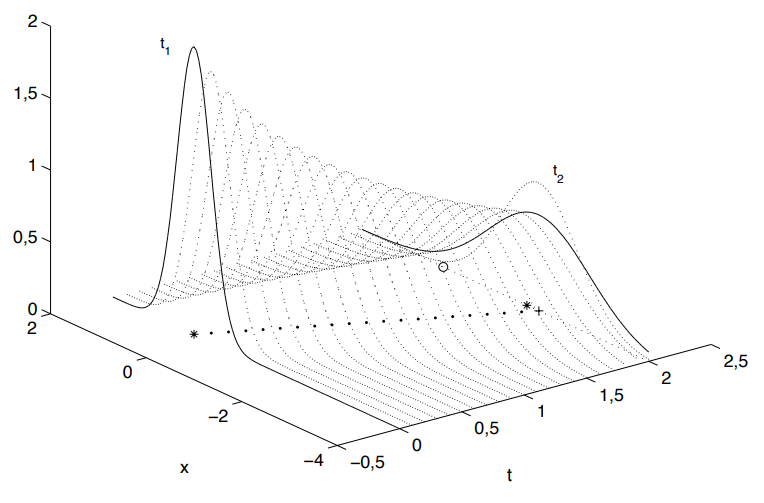
\includegraphics[width=0.5\textwidth]{images/pdf-propagacao.png}
	\end{figure}

\end{frame}

%------------------------------------------------

\begin{frame}
\frametitle{Estimação de Estados}
Considere o sistema dinâmico estocástico não-linear amostrado

\begin{equation*}\label{eq:processo}
\dot{x}(t)=f(x(t),u(t),w(t),t),
\end{equation*}
\begin{equation*}\label{eq:obs}
y(t_k)=g(x(t_k),v(t_k),t_k),
\end{equation*}
\vspace{0.3cm}
em que:
\vspace{0.4cm}

\begin{tabular}{l l}
	\hfill
	$x(t) \in \mathbb{R}^n$:  	& vetor de estados, \\
	\hfill
	$u(t) \in \mathbb{R}^p$:  	& vetor de entradas, \\
	\hfill
	$y(t_k) \in \mathbb{R}^m$ 	& vetor de observações, \\
	\hfill
	$w(t) \in \mathbb{R}^q$:	 	& ruído de processo, \\
	\hfill
	$v(t_k) \in \mathbb{R}^m$: 	& ruído de medição, \\
	\hfill
	$f$: 		& modelo de processo contínuo em $t$, \\
	\hfill
	$g$:  	 	& modelo de medição amostrado em $t_k$.
\end{tabular}

\end{frame}

%------------------------------------------------

\begin{frame}
	\frametitle{Modelo de Amostragem}
	
	Em geral, considera-se que os sinais são amostradas e disponibilizadas para o estimador a uma \textbf{taxa regular}.
	
	\vspace{0.5cm}
	
	No entanto, em muitas aplicações práticas, esse modelo não é verdadeiro:
	
	\begin{itemize}
		\item<2-> Limitações nos instrumentos ou na rede de comunicação
		\item<3-> Uso de muitos sensores redundantes, não sincronizados	
		\item<4-> Esquemas de amostragem baseado em eventos
		\item<5-> Aplicações industriais com medições laboratoriais
	\end{itemize}

\end{frame}

%------------------------------------------------

\begin{frame}
	\frametitle{Métodos para Amostragem Irregular}
	
	\textbf{Quando há carimbo de tempo}, pode-se optar pela aplicação de algum dos métodos disponíveis na literatura
	\begin{itemize}
		\item \textit{Custos computacionais}
	\end{itemize}
	
	\vspace{0.5cm}
	
	\textbf{Quando não há carimbo de tempo}, pode-se investir na sincronização temporal ou na utilização de GPS na rede
	\begin{itemize}
		\item \textit{Custos de infraestrutura}
	\end{itemize}

\end{frame}

%------------------------------------------------

\begin{frame}
	\frametitle{Objetivos}
	
	Custos adicionais valem a pena?
	\vspace{0.3cm}
	
	
	\begin{definicao}	
		\begin{itemize}
			\item Qual o efeito de se considerar o carimbo de tempo?
			\vspace{0.5cm}
			\item Quando vale a pena investir em sincronização ou em maior capacidade computacional?
			\vspace{0.5cm}
			\item Quais os fatores que impactam no desempenho do estimador?
		\end{itemize}
	\end{definicao}

\end{frame}

%------------------------------------------------

%------------------------------------------------SECTION---------------------------------
\section{Formulação do Problema} 
%------------------------------------------------

%------------------------------------------------

\begin{frame}
	\frametitle{Formulação do Problema}
	
	\begin{equation*}\label{eq:processo}
	\dot{x}(t)=f(x(t),u(t),w(t),t),
	\end{equation*}
	\begin{equation*}\label{eq:obs}
	y(t_k)=g(x(t_k),v(t_k),t_k),
	\end{equation*}
	\vspace{0.2cm}
	
	Assume-se que:
	
	\begin{itemize}
		\item $\forall k \geq 1$, $y(t_k) \in \mathbb{R}^m$ e $v(t_k) \in \mathbb{R}^r$ são conhecidos,
		\item $t_k$, $\forall k \in \mathbb{N^+}$, são ordenados ($t_{k+1}>t_k,\forall k \in \mathbb{N^+}$) e definidos pelos intervalos de tempo $h_0 \triangleq t_1$, $h_k \triangleq t_k-t_{k-1}, \ \forall k \geq 1$
		\item $u(t) \in \mathbb{R}^p$ são medidas em intervalos regularmente espaçados $T$ 
		\item $u(iT) \in \mathbb{R}^p$, $\forall i \geq 1$ são conhecidas
	\end{itemize}
	
	\vspace{0.3cm}
	
	$\rightarrow$ Deseja-se estimar o estado $x(iT)$ de forma recursiva, em intervalos regularmente espaçados $T$.

\end{frame}

%------------------------------------------------

\begin{frame}
	\frametitle{Formulação do Problema}
	Modelo de Amostragem Irregular:
	
	\begin{definicao}
		Os instantes de medição $t_k$ são dados por um processo aleatório de Poisson:
		
		\centering
		$h_k \sim \mathcal{E} (\lambda)$
	\end{definicao}
	
	\begin{figure}
		\centering
		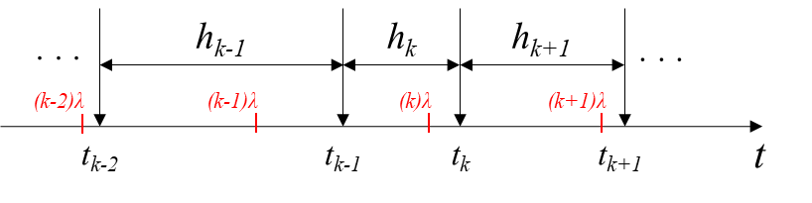
\includegraphics[width=0.75\textwidth]{images/processo_amost.png}
	\end{figure}
	
	\small
	\centering
	\textit{Esse modelo caracteriza uma aplicação comum para um sistema com rede de sensores dessincronizados \cite{Micheli2002}}

\end{frame}

%------------------------------------------------

%------------------------------------------------SECTION---------------------------------
\section{Metodologia} 


%------------------------------------------------

\begin{frame}
	\frametitle{Método de Estimação}
	
	Filtro de Kalman \textit{Unscented} (UKF) discreto \cite{Julier2004}
	
	\vspace{0.25cm}
	\begin{itemize}
		\item Discretização em instantes variáveis (com carimbo de tempo):	
		\begin{align*}
		&x(t^*_j)=f_{\textrm{d}}(x(t^*_{j-1}),u(t^*_{j-1}),w(t^*_{j-1}),t^*_{j-1}),\\
		&t^*_j= t^*_{j-1} + \delta t^*_j, \quad  t^*_0=0
		\end{align*}
		
		\vspace{0.25cm}
		\item Discretização em instantes regulares (sem carimbo de tempo):
		\begin{align*}
		&x_i=f^*_{\textrm{d}}(x_{i-1},u_{i-1},w_{i-1},i),\\
		&t=iT.
		\end{align*}
		
	\end{itemize}


\end{frame}

%------------------------------------------------

\begin{frame}
	\frametitle{Cenários de Estimação}
	
	\begin{figure}
		\centering
		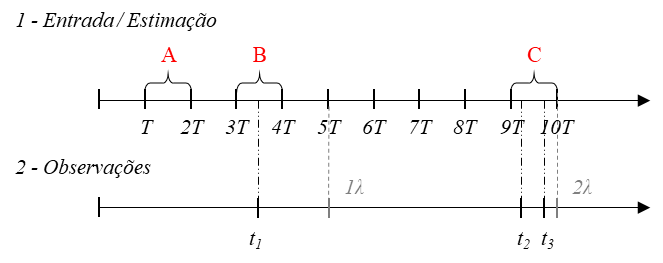
\includegraphics[width=0.75\textwidth]{images/cenarios-est.png}
	\end{figure}
	

\end{frame}

%------------------------------------------------SUBSECTION------------------------------

\subsection{Sem carimbo de tempo} 

\begin{frame}
	\frametitle{Sem carimbo de tempo}
	
	Só há dois cenários de estimação:
	\vspace{0.25cm}
	
	\begin{enumerate}
		\item Não há medições entre duas informações de entrada:
		\begin{itemize}
			\item Etapa de predição entre $iT$ e $(i+1)T$
		\end{itemize}
		\vspace{0.25cm}
		\item Há medições entre duas informações de entrada:
		\begin{itemize}
			\item Medição mais recente é assimilada no próximo instante de estimação, múltiplo de $T$
		\end{itemize}
	\end{enumerate}
	
	\textit{Passos de discretização são sempre $\delta t = T$}

\end{frame}

%------------------------------------------------

%------------------------------------------------SUBSECTION------------------------------

\subsection{Com carimbo de tempo} 

%------------------------------------------------

\begin{frame}
	\frametitle{Com carimbo de tempo}
	
	
	\begin{figure}
		\centering
		\begin{adjustbox}{width=\textwidth/2,height=0.8\textheight,keepaspectratio}
			
			\begin{tikzpicture}[node distance=2cm, font = \scriptsize]
			
			\node(start)[startstop][text width=3cm,align=center]{\textbf{Início} \\ $t^*_0=0$; \\ $i=j=k=1$; \\};
			
			\node (dec1) [decision, below of=start,yshift=-0.5cm] {Sinal Recebido};
			
			\node (pro1) [process, below right of=dec1, yshift=-0.7cm, xshift=0.25cm][text width=3cm,align=center]{Calcula \\ $\delta t^*_{j} = iT - t^*_{j-1}$ \\ $t^*_{j} = t^*_{j-1} + \delta t^*_{j}$};
			
			\node (pro12) [process, below of=pro1][text width=3cm,align=center, yshift=0.5cm]{Etapa de Predição};
			
			\node (pro2) [process, below left of=dec1,  yshift=-0.7cm, xshift=-0.25cm][text width=3cm,align=center]{Calcula \\ $\delta t^*_{j} = t_k - t^*_{j-1}$ \\ $t^*_{j} = t^*_{j-1} + \delta t^*_{j}$};
			
			\node (pro22) [process, below of=pro2][text width=3cm,align=center, yshift=0.5cm]{Etapa de Predição, utilizando ZOH};
			
			\node (pro23) [process, below of=pro22][text width=3cm,align=center, yshift=0.5cm]{Etapa de Assimilação de Dados};
			
			\node (pro3) [startstop, below of = pro23][text width=3cm,align=center, xshift=1.8cm]{Estimativa em $t^*_{j}$};
			
			\draw [arrow] (start) -- node[pos=0.5](h){} (dec1);
			\draw [arrow] (dec1) -| node[text width=3cm,align=center,anchor=west,xshift=-1cm] {Sinal de \\ Entrada} (pro1);
			\draw [arrow] (dec1) -| node[text width=3cm,align=center,anchor=east,xshift=0.8cm] {Sinal de \\ Observação} (pro2);
			\draw [arrow] (pro1) -- (pro12);
			\draw [arrow] (pro2) -- (pro22);
			\draw [arrow] (pro22) -- (pro23);
			\draw [arrow] (pro12) -- node[text width=3cm,align=center,anchor=south,xshift=1cm] {$i=i+1$} (pro3);
			\draw [arrow] (pro23) -- node[text width=3cm,align=center,anchor=east,xshift=0.6cm] {$k=k+1$}(pro3);
			\draw [arrow] (pro3) --+(-4cm,0) |- node[text width=3cm,align=center,anchor=south,xshift=1cm] {$j=j+1$}(h);
			\end{tikzpicture}
		\end{adjustbox}
	\end{figure}	


\end{frame}

%------------------------------------------------


%------------------------------------------------SECTION---------------------------------
\section{Resultados Simulados} 
%------------------------------------------------SUBSECTION------------------------------

\subsection{Descrição do Sistema} 

%------------------------------------------------

\begin{frame}
	\frametitle{Descrição do sistema}
	Considere o sistema de um robô móvel não-holonômico:

	\begin{minipage}{.70\textwidth}
		\begin{equation*}
					\begin{split}
		\dot{p}_{\textrm{x}} & = v\cos (\theta),\\
		\dot{p}_{\textrm{y}} & = v\sin (\theta),\\
		\dot{\theta}  & = u_1(t),\\
		\dot{v} & = u_2(t),
		\end{split}
		\end{equation*}
		
			
		em que:
		
		\vspace{0.2cm}
		
		\centering
		
		\begin{tabular}{l l}
			\hfill
			$p_{\textrm{x}}$ e $p_{\textrm{y}}$:	& coordenadas de posição, \\
			\hfill
			$\theta$:  							& orientação angular, \\
			\hfill
			$v$:								& velocidade linear, \\
			\hfill
			$u_1$:	 							& entrada: velocidade angular ($\omega$), \\
			\hfill
			$u_2$:	 							& entrada: aceleração linear ($a$)
		\end{tabular}
		
	\end{minipage}%
	\begin{minipage}{.3\textwidth}
	\begin{figure}
		\centering
		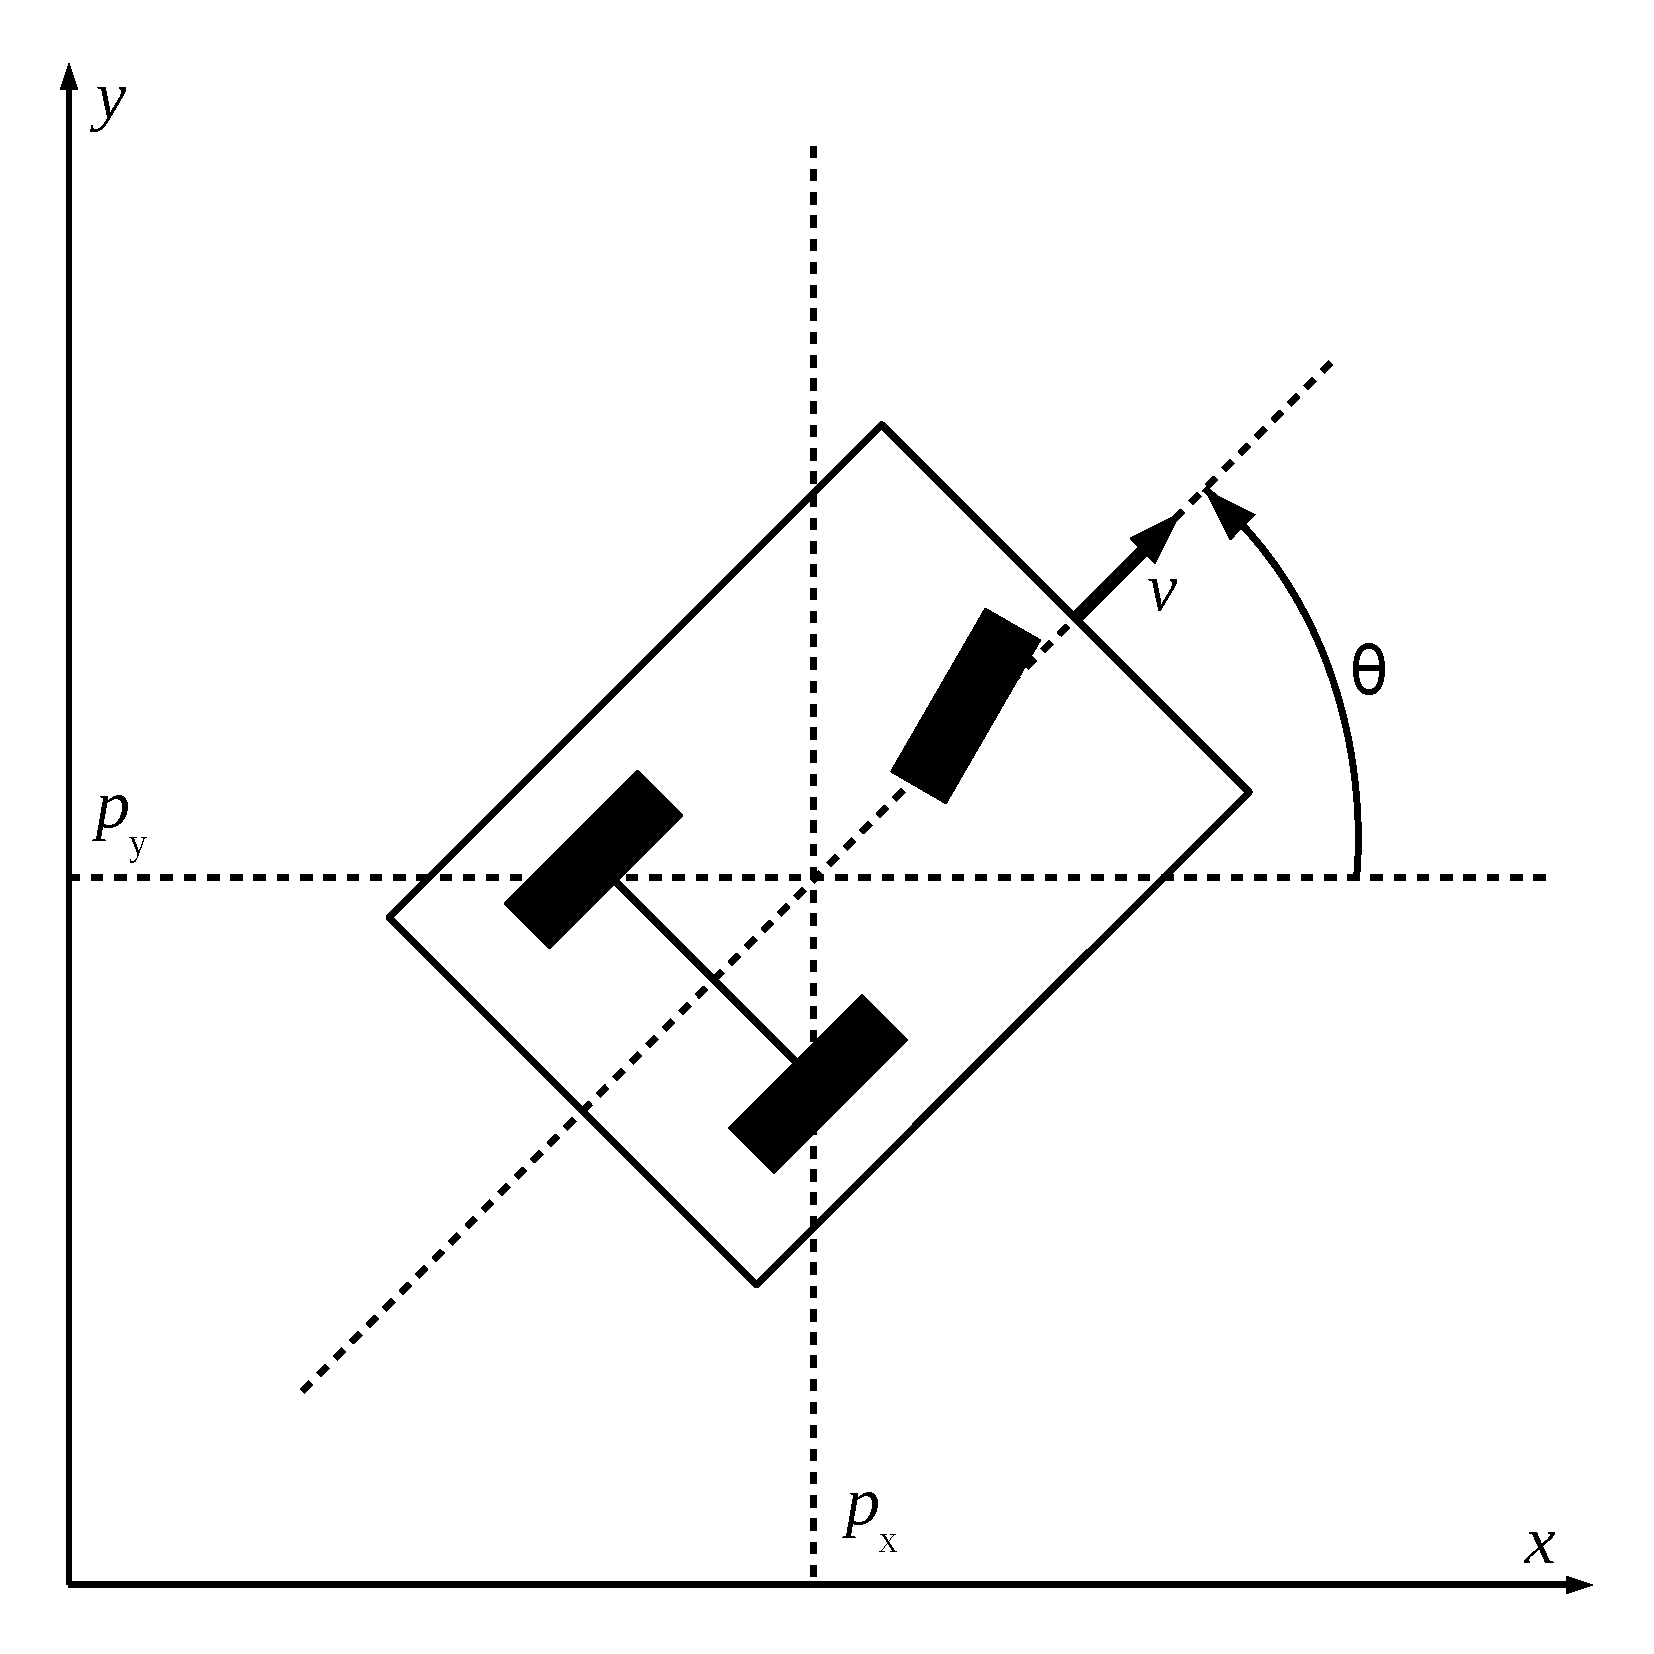
\includegraphics[width=1\textwidth]{images/Nonholomonic-robot.pdf}
	\end{figure}
\end{minipage}



\end{frame}

%------------------------------------------------


\begin{frame}
	\frametitle{Robô Móvel não-Holomônico}
	
	Vetor de estados:
	\begin{equation*}
	x_i \overset{\Delta}{=} [p_{\textrm{x},i}\ p_{\textrm{y},i}\ \theta_i\ v_i]^T.
	\end{equation*}
	
	\vspace{0.25cm}
	Modelo de observações:
	\begin{equation*}
	y(t_k) = 
	\begin{bmatrix}
	p_{\textrm{x}}(t_k) \\
	p_{\textrm{y}}(t_k)
	\end{bmatrix}+v(t_k),
	\end{equation*}
	\begin{equation*}
	v(t_k) \sim \mathcal{N} (0,R_{t_k}).
	\end{equation*}
	
	\vspace{0.25cm}
	Vetor de entradas:
	\begin{equation*}
	u_i = [\omega_i\ a_i]^T,
	\end{equation*}
	\begin{equation*}
	u_i = \tilde{u}_i - w_i,
	\end{equation*}
	\begin{equation*}
	w \sim \mathcal{N} (0, Q_i).
	\end{equation*}


\end{frame}

%------------------------------------------------

\begin{frame}
\frametitle{Parâmetros da Simulação}

\begin{itemize}
	\item 60 segundos de simulação
	\vspace{0.25cm}
	\item $\delta t_{\textrm{sim}} = 10^{-4}$
	\vspace{0.25cm}
	\item $h_k$ calculado usando $\textrm{exprnd()}$ do MatLab\texttrademark e aproximado entre os 600.000 pontos de simulação
	\vspace{0.25cm}
	\item 100 realizações foram realizadas para cada cenário de simulação. A média e o IC 95\% são apresentados
	\vspace{0.25cm}
	\item Índice de desempenho utilizado:
	
	\begin{equation*}
	J = \frac{ \sum_{i=1}^N \sqrt{(\hat{p}_{\textrm{x},i}-p_{\textrm{x},i})^2+(\hat{p}_{\textrm{y},i}-p_{\textrm{y},i})^2}}{N}
	\end{equation*}
	
\end{itemize}

\end{frame}
%------------------------------------------------

\begin{frame}
\frametitle{Entradas}

	\begin{figure}
		\centering
		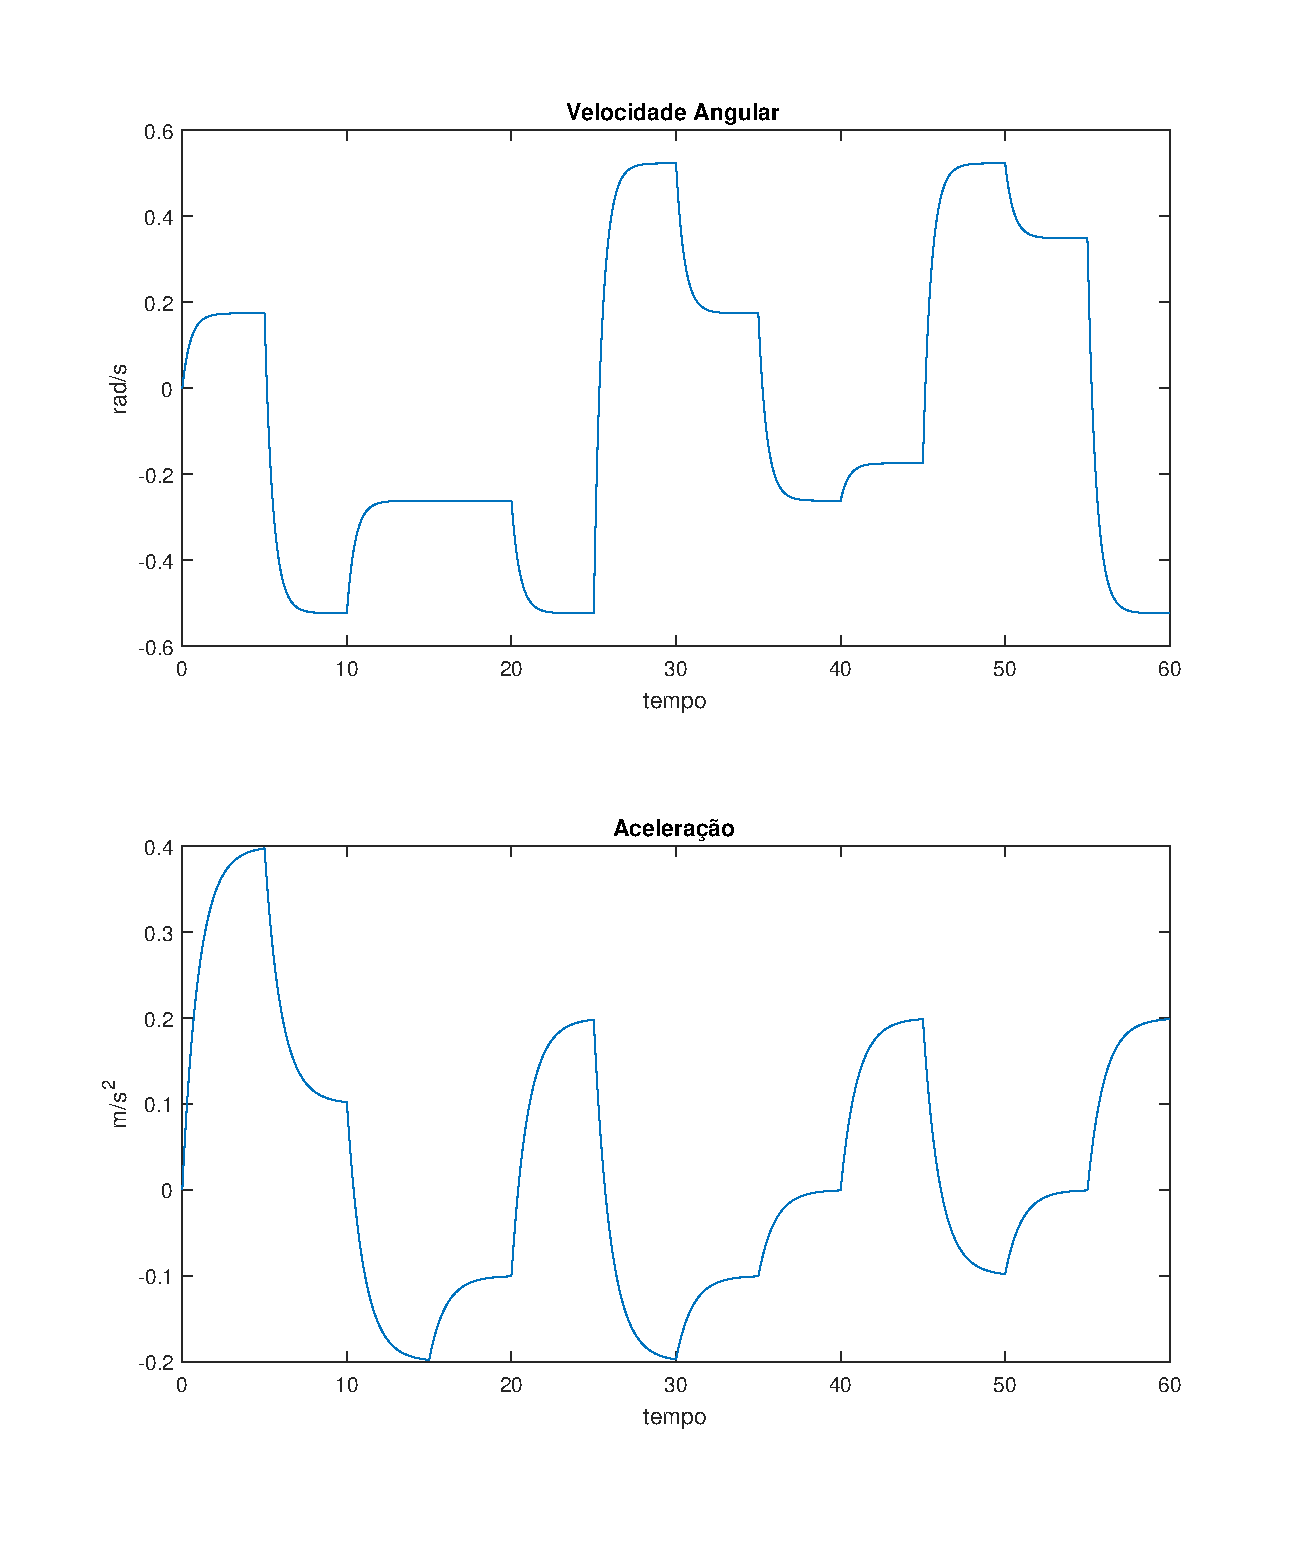
\includegraphics[width=0.5\textwidth]{images/entradas.eps}
	\end{figure}

\end{frame}
%------------------------------------------------

\begin{frame}
\frametitle{Exemplo de Realização}

\begin{figure}
	\centering
	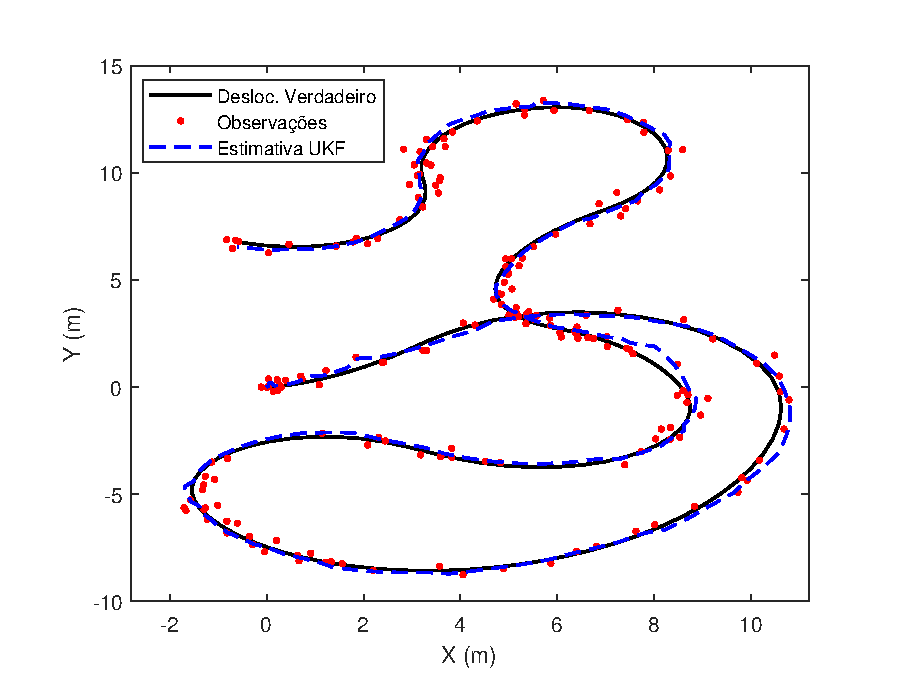
\includegraphics[width=0.75\textwidth]{images/exemplo_03_30db_desloc.eps}
\end{figure}

\end{frame}
%------------------------------------------------


%------------------------------------------------

%
%
%O sistema descrito por~\ref{eq:sistema} é discretizado por meio do método de Runge-Kutta de 4ª ordem e o vetor de estados $x_i$ é dado por $x_i \overset{\Delta}{=} [p_{\textrm{x},i}\ p_{\textrm{y},i}\ \theta_i\ v_i]^T$.
%
%
%O modelo de observações é dado por
%
%\begin{equation}
%y(t_k) = 
%\begin{bmatrix}
%p_\textrm{x}(t_k) \\
%p_\textrm{y}(t_k)
%\end{bmatrix}+v(t_k), \\
%\end{equation}
%
%\noindent
%em que $v(t_k) \sim \mathcal{N} (0,R_{t_k})$ é o ruído de observação com média nula e covariância $R_{t_k}$. Para o cenário sem carimbo de tempo, o vetor de observações é aproximado por $\tilde{y}_i \approx y(t_k)$, em que $i$ é o índice do próximo instante de tempo múltiplo de $T$.
%
%O vetor de entradas $u_i = [\omega_i\ a_i]^T$, é medido por meio de girômetro e acelerômetro, respectivamente. Assume-se que
%
%\begin{equation}\label{eq:entrada}
%u_i = \tilde{u}_i - w_i,
%\end{equation}
%
%\noindent
%em que $\tilde{u}$ é o valor medido pelos sensores e $w \sim \mathcal{N} (0, Q_i)$ representa o ruído correspondente, de média nula e covariância $Q_i$.

%------------------------------------------------SUBSECTION------------------------------

\subsection{Resultados} 


\begin{frame}
	\frametitle{Cenários Simulados}
	
	\begin{enumerate}
		\item Variação do nível de ruído de observação
		\vspace{0.5cm}
		\item Variação do intervalo médio de amostragem	de observação ($\lambda$)
		\vspace{0.5cm}
		\item Variação da relação entre intervalo médio de amostragem de observação e intervalo regular de estimação $\alpha=T/\lambda$
	\end{enumerate}

\end{frame}
%------------------------------------------------


%------------------------------------------------

\begin{frame}
	\frametitle{Nível de Ruído das Medições}
	
	\begin{figure}
		\centering
		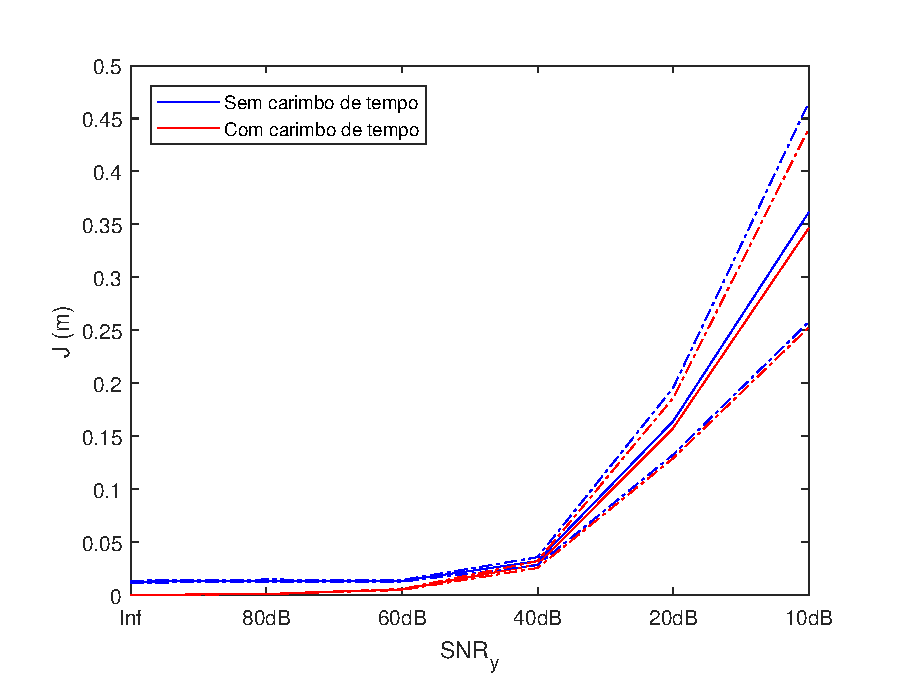
\includegraphics[width=0.75\textwidth]{images/noise.eps}
	\end{figure}


\end{frame}
%------------------------------------------------

\begin{frame}
	\frametitle{Intervalo Médio das Medições}
	
	\begin{figure}
		\centering
		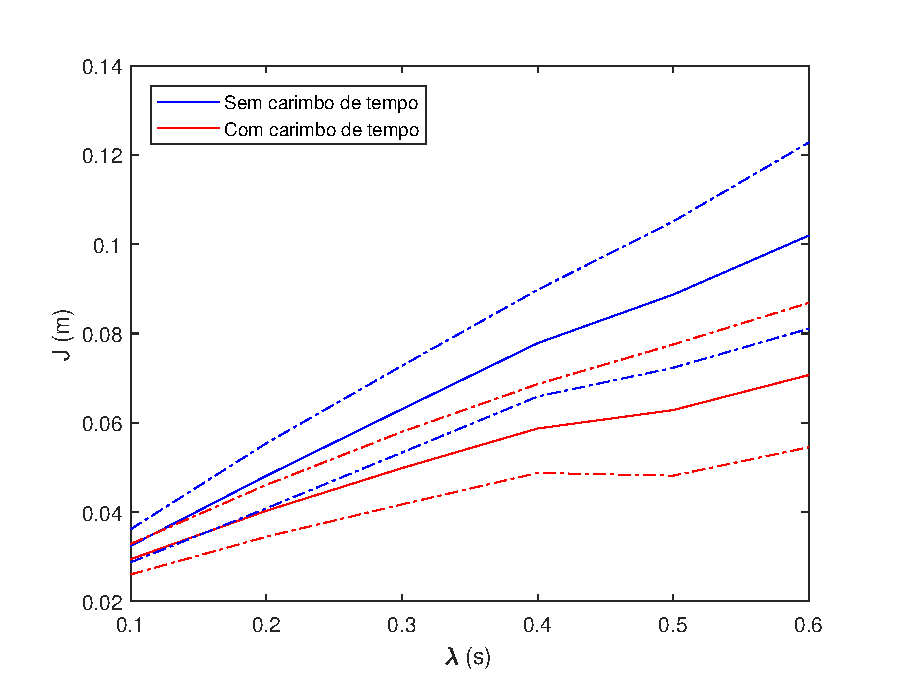
\includegraphics[width=0.75\textwidth]{images/samp.eps}
	\end{figure}

\end{frame}

%------------------------------------------------

\begin{frame}
	\frametitle{Relação $\alpha = T/\lambda$}
	
	\begin{figure}
		\centering
		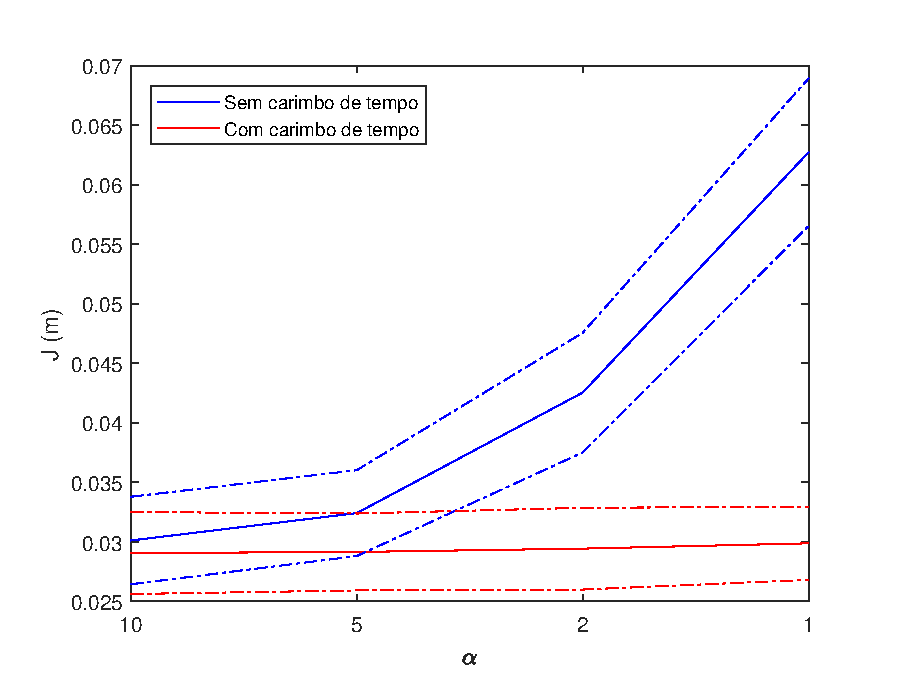
\includegraphics[width=0.75\textwidth]{images/dtudty.eps}
	\end{figure}

\end{frame}

%------------------------------------------------

%------------------------------------------------SECTION------------------------------

\section{Conclusões} 

\begin{frame}
	\frametitle{Conclusões}
Abordagem útil para a tomada de decisão sobre investir em sincronização e capacidade computacional.
\vspace{0.2cm}

O investimento pode não valer a pena para:
	
	\begin{itemize}
		\item Sistemas cujo \textbf{modelo de processo apresenta pouco ruído} em relação ao ruído de observações 
		\item Sensores de \textbf{observação} com \textbf{alta frequência de amostragem} em relação à dinâmica do sistema
		\item Sensores dos \textbf{sinais de entrada} com \textbf{alta frequência de amostragem} em relação à frequência dos sensores de observação
	\end{itemize}

\end{frame}

%------------------------------------------------


{
\setbeamertemplate{footline}{}
\usebackgroundtemplate{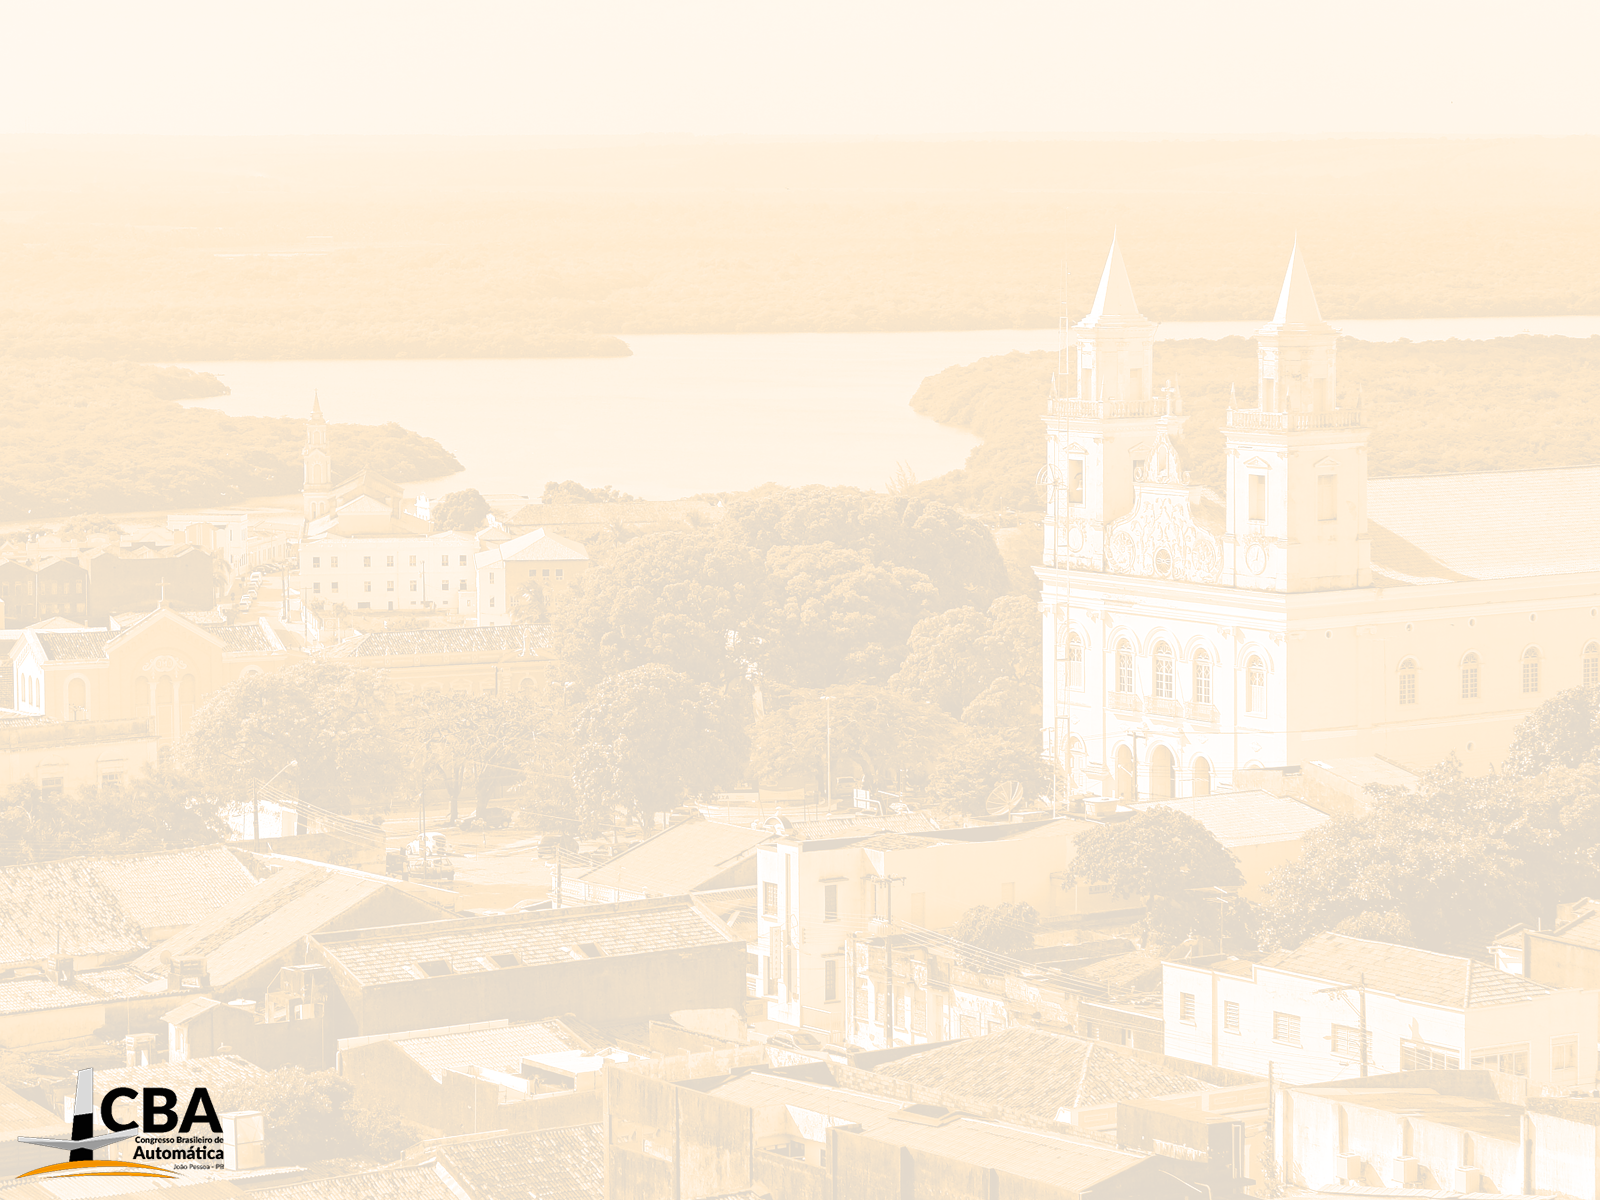
\includegraphics[width=\paperwidth]{template/fim.png}}%
\begin{frame}[plain]
\centering
\Large
\textbf{Obrigado!}

\vspace{1cm}
\normalsize
\href{tatatupi@gmail.com}{tatatupi@gmail.com}

\end{frame}
\addtocounter{framenumber}{-1}

}



\end{document}


